\chapter{Proposition of new model}

\label{chap:research}

We aimed to create new semi-supervised model which include concept of self-organization in uninformed part of semi-supervised model. This chapter contains selection of self-organizing model, our first design of new semi-supervised model and its drawbacks and proposition of final design of the new model, which will be fine tuned in following chapters.

Unsupervised loss in semi-supervised learning is mostly based on prediction consistency. In case of Mean Teacher model, this consistency is between predictions of teacher and student model. Other models, for example Siamese neural network, holds consistency between predictions of one model on sample augmented in two different ways.

\section{Unsupervised model selection}
In our research, we decided to use Self-organizning map (SOM) as model of consistency of data points from same class. Self-organizning map was described in section \ref{sec:som}. SOM was used as unsupervised component of loss function. Unlike other unsupervised techniques, SOM can provide nonlinear transformation of the input and it is neural network based, so its complexity is scalable. We expected that clustering using SOM can be usefull to determine similarity of training examples.



\section{Related work}

\subsection{DESOM model}

Forest et al. \cite{desom2019} introduced introduced model called  Deep Embedded Self-Organizing Map (DESOM). Authors combined two unsupervised models - autoencoder and SOM. Combined model is trained in unsupervised setup and has really good results in clustering task. Clusters are taken from SOM part of model. It is first ever usage of SOM in deterministic autoencoder model. Proposed model architecture is described in figure \ref{fig:desom}. 


\begin{figure}[h!]
        \centering
        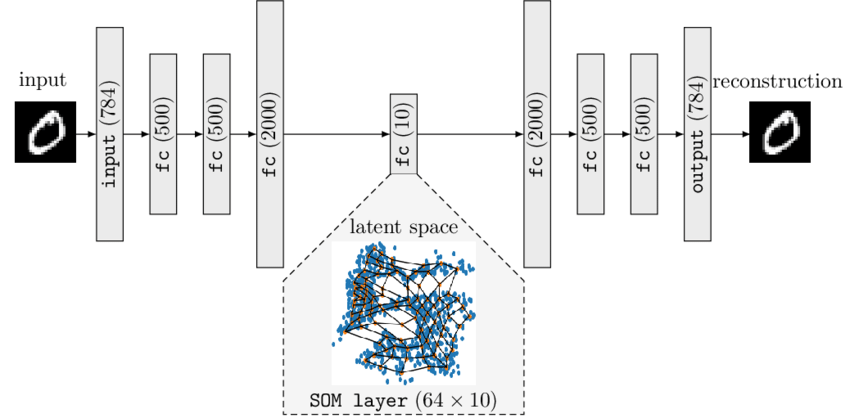
\includegraphics[width=1\textwidth]{figs/DESOM-architecture-with-an-8-8-map.png}
        \caption{DESOM model architecture \cite{desom2019}}
        \label{fig:desom}
\end{figure}

DESOM model uses combined loss in encoder network training - weighted sum of reconstruction loss $\mathcal{L}_r$ (which is standardly used in autoencoder) and SOM loss $\mathcal{L}_{som}$.
SOM loss is defined as $$\mathcal{L}_{som} = \sum_i \sum_{k=1}^K \mathcal{K}^T (\delta (\mathcal{X}(f_{W_e}(x_i)), k)) {||f_{W_e}(x_i) - m_k||}^2$$. Where neurons in SOM are numbered from $1$ to $\mathcal{K}$ and weights of $k$-th neuron (prototype) are denoted $m_k$. $\mathcal{K}^T$ is neighbour function dependant on time $T$ which computes neighbourhood relationship based on difference $\delta$ between $k$-th neuron and winner neuron in SOM $\mathcal{X}(f_{W_e}(x_i))$ for $i$-th input.
Decoder part is trained only using $\mathcal{L}_r$. SOM is trained using $\mathcal{L}_{som}$. Authors used no pretraining.

In their experimental part, they focused on unsupervised clustering accuracy (using SOM part of model), in which DESOM has best results in all three datasets (MNIST, Fashion-MNIST, REUTERS-10k). They also examined Purity and NMI matrices, in which they model compared with other clustering models achieved best in majority of the cases best results.

This article brings us $3$ findings important for our reseach. First, that it is possible to use some kind of extracted information (latent space representation of autoencoder) as input for SOM and the results are really good. Second, it is possible to train SOM on changing inputs and it still clusters data properly. And third, usage of another model can impove model in its task. These results support our intuition, that self-organization of data can also improve performance of semi-supervised model.


\subsection{}
\color{red}Increasing the share of correct clustering of characteristic signal with random losses in self-organizing maps
\color{black}

\section{Our first approach}
We extended semi-supervised model Mean Teacher described in section \ref{mtm-chapter}. Our model is described in details in figure \ref{fig:our-model}. We suggested to replace original unsupervised loss of the model by using distances of winner neurons in SOM. The inputs to SOM are feature vectors from Mean Teacher model. The distance between winner neurons was computed as euclidian distance of weights of selected winner neurons in multidimensional space. Other parts of MT model did not change. Lets denote weight vector of winner neuron of student $x^{1}$ and weight vector of winner neuron of teacher $x^{2}$. Consistency loss can be then computed as $$J(\theta) = \sqrt{\sum_{i=1}^n {(x^1_i - x^2_i)}^2}.$$ 
\begin{figure}[h!]
    \centering
    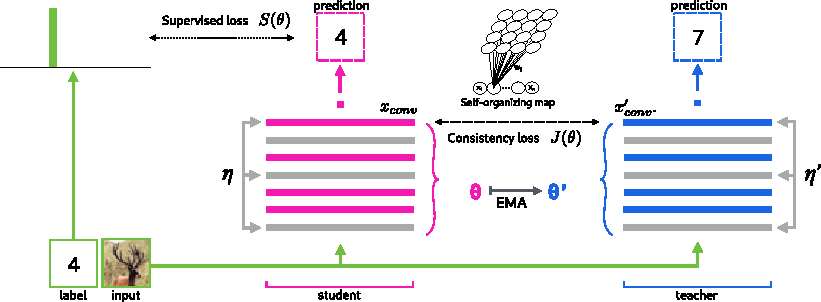
\includegraphics{figs/mean_teacher_som-1.pdf}
    \caption{Description of our model}
    \label{fig:our-model}
\end{figure}


\color{red} zjednotit oznacenia v rovnici a obrazku !!!!! \color{black}

\subsection{Feature vector usage}
Idea of using feature vectors instead of predictions for unsupervised cost is from \cite{tuna-bmt} and it is supported by \cite{desom2019}. We decided to use it, since it worked well for BMT model and we believed it can contain more information than prediction, because it has higher dimension than output vector and still contains only extracted features that are important for classification.

To strenghten our intuition, that SOM is able to cluster MT feature vectors properly, we took implemetation of Mean Teacher from authors Github repository \footnote{https://github.com/CuriousAI/mean-teacher} and produced feature vectors for setup that declared state-of-the-art results. The input dataset for MT was standard dataset CIFAR10 previously described in section \ref{dataset-cifar10}, which contains color images from $10$ classes. Then we used feature vectors as inputs for SOM. SOM was trained in unsupervised setup for $30$ epochs and the two dimensional map is was visualized in figure \ref{fig:som-cluster-mt}. We can see that neurons are quite well organised. Further investigation of difference between original CIFAR10 versus feature vectors from MT as the input is in chapter \ref{chap:som-fv-cifar}.

\begin{figure}[h!]
    \centering
    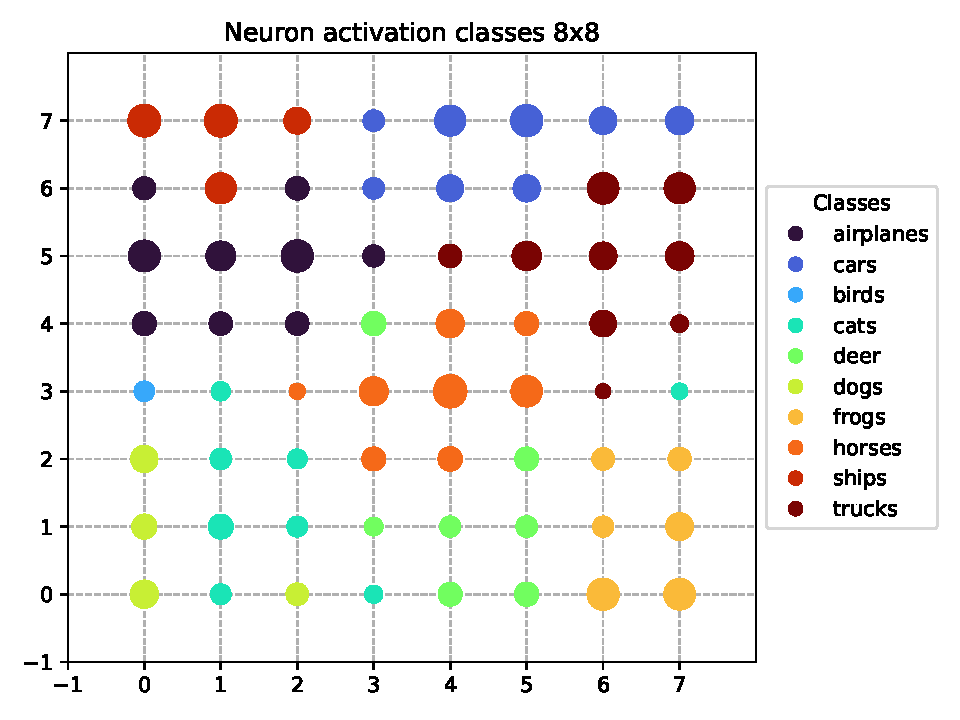
\includegraphics[width=0.9\textwidth]{figs/som-clusters-mt.pdf}
    \caption[Som clusters from MT feature vectors]{In the legend, we can see 10 classes of dataset CIFAR-10. Dots in the graph show properties of neurons in $8\times8$ grid. Color means class which neuron represents and size means portion of input vectors of this class that are represented by this neuron. We can see, that space is organized into clusters and all inanimate object clusters are in the upper part. Animate object clusters are in the lower part. Also we can see that cluster of airplanes is right next to neuron that represents birds. We cas see an outlayer from the deer class in the middle, but we can explain it by looking what is in between of this oulayer and deer cluster. It is a horse cluster, so since these creatures are quite similar, it can be explanation of this outlayer.}
    \label{fig:som-cluster-mt}
\end{figure}


\newpage

\subsection{Problems of straight-forward implementation}

To prove our new concept we designed experimental setup for semisupervised CIFAR10 classification. We used MT implementation and hidden layer architecture from authors of MT, that is available in Github repository \footnote{\url{https://github.com/CuriousAI/mean-teacher}}. Since implementation of MT is in Pytorch framework, we considered several SOM implementations and select one which is available in this GitHub repository \footnote{\url{https://github.com/giannisnik/som}}.
Our experiment implementation is available in another repository \footnote{\url{https://github.com/sabka/dt-mt}}. Since this architecture of MT model has approximately $30$ milions parametres, we were not able to run optimisation of hyperparameters in reasonable amount of time. We tried another architecture, from Sarmads repository\footnote{\url{https://github.com/iSarmad/MeanTeacher-SNTG-HybridNet/}}, with approximately $3$ milion parametres. During our early experiments, we found out, that supervised pretraining of MT is crucial. Without pretraining (5 epochs were enough) MT did not increase training accuracy. Model was still too complex and we were unable to investigate all the hyperparameter options with our computational performance.
\color{red} TREBA SA POZRIET NA KOD A SFINALIZOVAT ! otestovat, ci sa to trenuje alebo nie, oddelit baseline, dat ako samostatny exp !!! \color{black}

\color{red} pravda je, ze kod dava nan pri SOM metrikach aj SOM loss, moj tip je ze je zla somka \color{black}

\color{red} prvych 30 epoch training acc stupa, a overfitne na skoro 100 percent, val acc ostava na cca 60 percent a nejde hore\color{black}

\color{red} 31. epocha -> pouzivame pevne dane num of iters 30, ale ako cislo iteracie pride cislo epochy MT \color{black}

\color{red} fixla som nany, asi, davam kappa = 1/500, som trenujem od 0. epochy ale pouzivam az po 3 epochach \color{black}

\color{red}cez noc - 180 epoch, rychlo overfitne a skonci na 100 trenovacej a 50ish test \color{black}


\section{Our second approach}
Based on previous small experiments, we decided to redefine our model.
We decided to create model based on two main components: unsupervised loss based on self-organization representation of data in and usage of feature vectors from semisupervised mean teacher model.

pretrained SOM na FV z MT (5\% CIFAR10)
→ 
MLP + som loss (zase trojicky)


\color{red} TODO \color{black}
